\documentclass[tikz,border=5pt]{standalone}
\usepackage{amsmath}
\usepackage{pgfplots}
\begin{document}

\begin{figure}[h]
\begin{center}
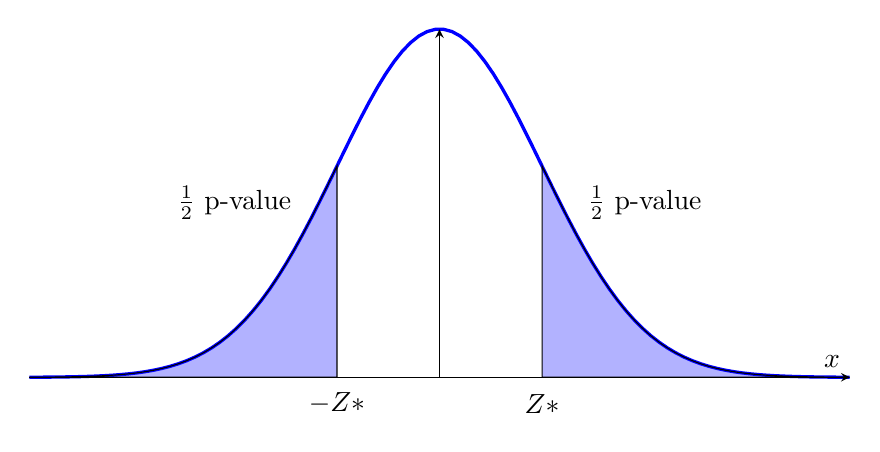
\begin{tikzpicture}
  \begin{axis}[
    no markers, domain=-4:4, samples=100,
    axis lines=middle,
    xlabel={$x$}, ylabel={},
    height=6cm, width=12cm,
    xtick=\empty,
    ytick=\empty,
    enlargelimits=false, clip=false,
    axis on top,
    grid = major,
  ]
    \addplot [very thick, blue] {1/sqrt(2*pi) * exp(-x^2/2)};
    \addplot [
      domain=-4:-1,
      samples=100,
      fill=blue,
      fill opacity=0.3,
    ]
    {1/sqrt(2*pi) * exp(-x^2/2)} \closedcycle;
    \addplot [
      domain=1:4,
      samples=100,
      fill=blue,
      fill opacity=0.3,
    ]
    {1/sqrt(2*pi) * exp(-x^2/2)} \closedcycle;

    % Labels for p-value regions
    \node at (axis cs:-2,0.2) {$\frac{1}{2}$ p-value};
    \node at (axis cs:2,0.2) {$\frac{1}{2}$ p-value};
    \node at (axis cs:1, -0.03) {$Z*$};
    \node at (axis cs:-1, -0.03) {$-Z*$};
  \end{axis}
\end{tikzpicture}
\end{center}
\caption{An illustration of hypothesis test on a proportion that $H_0: p = p_0$, $H_a: p \neq p_0$.}
\end{figure}
\end{document}